游戏开发是软件工程中最有趣的话题之一。C++因其高效而广泛应用于游戏开发中,但由于言没有GUI组件,所以在后端使用。本章中,我们将学习如何在后端设计策略游戏。我们将把前面章节中学到的所有东西都结合起来,包括设计模式和多线程。 \par
我们要设计的游戏是一款名为《读者与扰乱者》的策略游戏。玩家创造了能够建造图书馆和其他建筑的单位,也就是所谓的“读者”,以及守卫这些建筑不受敌人攻击的士兵。 \par
本章中,我们将了解以下内容: \par

\begin{itemize}
	\item 游戏制作入门
	\item 深入研究游戏设计过程
	\item 使用设计模式
	\item 设计游戏循环
\end{itemize}

\noindent\textbf{}\ \par
\textbf{编译器要求} \ \par
g++编译器需要添加编译选项 \texttt{-std=c++2a} 来编译本章的代码。可以从这里获取本章的源码文件:https:/​/github.​com/PacktPublishing/Expert-CPP \par

\noindent\textbf{}\ \par
\textbf{游戏制作入门} \ \par
这章中,我们将设计一款策略游戏的后端,玩家可以创建单位(工人,士兵),建造建筑,并与敌人战斗。设计一款游戏,无论是战略游戏还是第一人称射击游戏,都有一些基本元素是相同的,比如:游戏物理元素,能够让玩家觉得游戏更真实,更有沉浸感。 \par
游戏设计中有些组件会在所有游戏中重复出现,如:碰撞检测机制、音频系统、图像渲染等。设计游戏时,我们既可以区分引擎和游戏,也可以开发一个紧密结合的应用程序,将引擎和游戏作为单独的成果。单独设计的游戏引擎,需要允许为进一步开发进行扩展,甚至用于其他游戏。毕竟,游戏都有相同的机制和流程。他们的不同之处在于情节主线。 \par
设计游戏引擎时,应该仔细规划使用该引擎的游戏类型。独立于游戏类型之外,3D射击游戏和策略游戏也有区别。策略游戏中,玩家在一个大的游戏场地上,有策略地部署单位。游戏世界是以自上而下的视角呈现的。 \par

\noindent\textbf{}\ \par
\textbf{了解《读者与扰乱者》游戏} \ \par
这款游戏很简单:玩家拥有有限的资源。这些资源可以用来为游戏角色创造建筑。我们将角色单位命名为读者和士兵。读者是建造图书馆和其他建筑的人物。每个构建的库最多可以容纳10个读者。如果玩家将10个读者移进图书馆,在一段特定时间后,图书馆将产生1个教授。教授是一个强大的单位,可以摧毁三个敌人。教授可以为士兵创造更好的武器。 \par
游戏一开始有一座已经建好的房子,两个士兵和三个读者。一所房子每5分钟生产一个新的读者。读者可以建造新的房子,这样就能产生更多的读者。他们也可以建造兵营来生产士兵。 \par
玩家的目标是建立5个库,每个库至少有一个教授。玩家必须在游戏中保护他/她的建筑和读者不受敌人攻击。敌人称为干扰者,因为他们的目标是干扰读者在图书馆里学习。 \par

\noindent\textbf{}\ \par
\textbf{战略游戏组件} \ \par
我们的策略游戏将包含基本组件——读者和士兵(称为单位)、建筑和地图。游戏地图包含游戏中每个对象的坐标。我们将讨论一个更轻版本的游戏地图。现在,让我们利用设计技能分解游戏本身. \par
游戏由以下角色单位组成: \par

\begin{itemize}
	\item 读者
	\item 士兵
	\item 教授
\end{itemize}

它还包括以下建筑物: \par

\begin{itemize}
	\item 图书馆
	\item 房子
	\item 兵营
\end{itemize}

现在,让我们讨论游戏中每个组件的属性。游戏角色有以下属性: \par

\begin{itemize}
	\item 生命值(整数,每次敌人攻击后会减少)
	\item 攻击力(整数,可以对敌人单位造成的伤害)
	\item 角色(读者,士兵,教授)
\end{itemize}

生命值应该有一个基于单位类型的初始值。例如,读者的初始生命值是10,而士兵的初始生命值是12。当在游戏中,所有的单位都可能受到敌人单位的攻击。每次攻击描述为生命点的减少。我们将减少的生命点数是基于攻击者的攻击力。例如,士兵的攻击力设置为3,这意味着士兵的每一次攻击都会让生命值减少3点。当受攻击的单位生命值小于等于0时,单位将死亡。 \par
建筑也是如此。建筑物有一个建造周期,一个建筑物也有生命值,任何敌人对建筑造成的伤害都会降低这些生命值。以下是建筑物业的完整列表: \par

\begin{itemize}
	\item 生命值
	\item 建筑类型
	\item 建造时间
	\item 生产时间
\end{itemize}

生产单位持续时间是指,生产一个新角色单位所需要的时间。例如,一个兵营每3分钟产生一个士兵,一个房子每5分钟产生一个读者,一个图书馆在10个读者进入图书馆时立即产生一个教授。 \par
现在定义了游戏组件,让我们来讨论它们之间的交互作用。 \par

\noindent\textbf{}\ \par
\textbf{组件之间的相互作用} \ \par
游戏设计的下一个重要内容是角色之间的互动。我们已经提到,读者可以建造建筑物。游戏中,这一过程应该得到重视,因为每种类型的建筑都有其建造时间。因此,如果读者正忙于构建过程,我们应该计算时间,以确保构建将在指定的时间后完成。然而,为了让游戏变得更好,我们应该考虑到不止一个读者可以参与到构建过程中。这应该会使建造楼房的速度加快。例如,如果一个兵营是一个读者需要5分钟建造的,那么两个读者就应该在2.5分钟完成,以此类推。这是游戏中复杂互动的一个例子,可以用下图来描述: \par

\begin{center}
	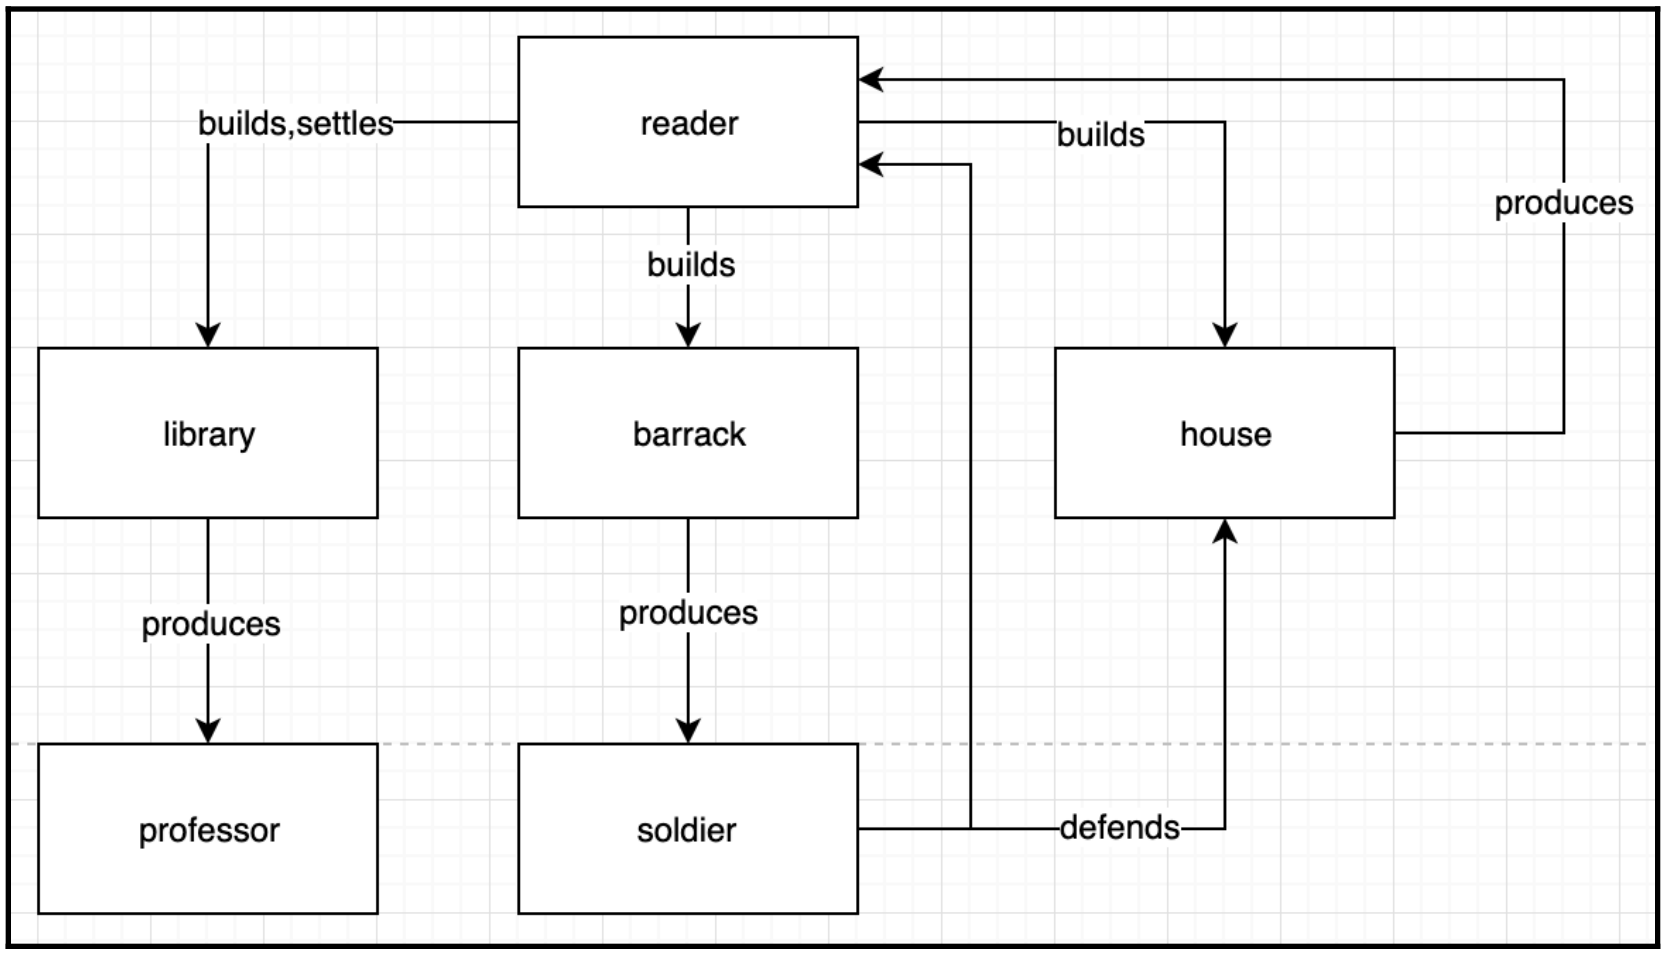
\includegraphics[width=1.0\textwidth]{content/Section-2/Chapter-11/1}
\end{center}

接下来是处理攻击。当一个单位遭受攻击时,我们应该减少单位的生命值。单位可以进行反攻(保护自己)。当有多个攻击者或防御者时,我们应该应该对每次攻击都进行处理。还定义单位每次命中的持续时间,一个单位不应该快速攻击另一个单位。为了让事情更自然,我们会在每次点击之间引入1秒或2秒的暂停。下图描述了一个简单的攻击交互: \par

\begin{center}
	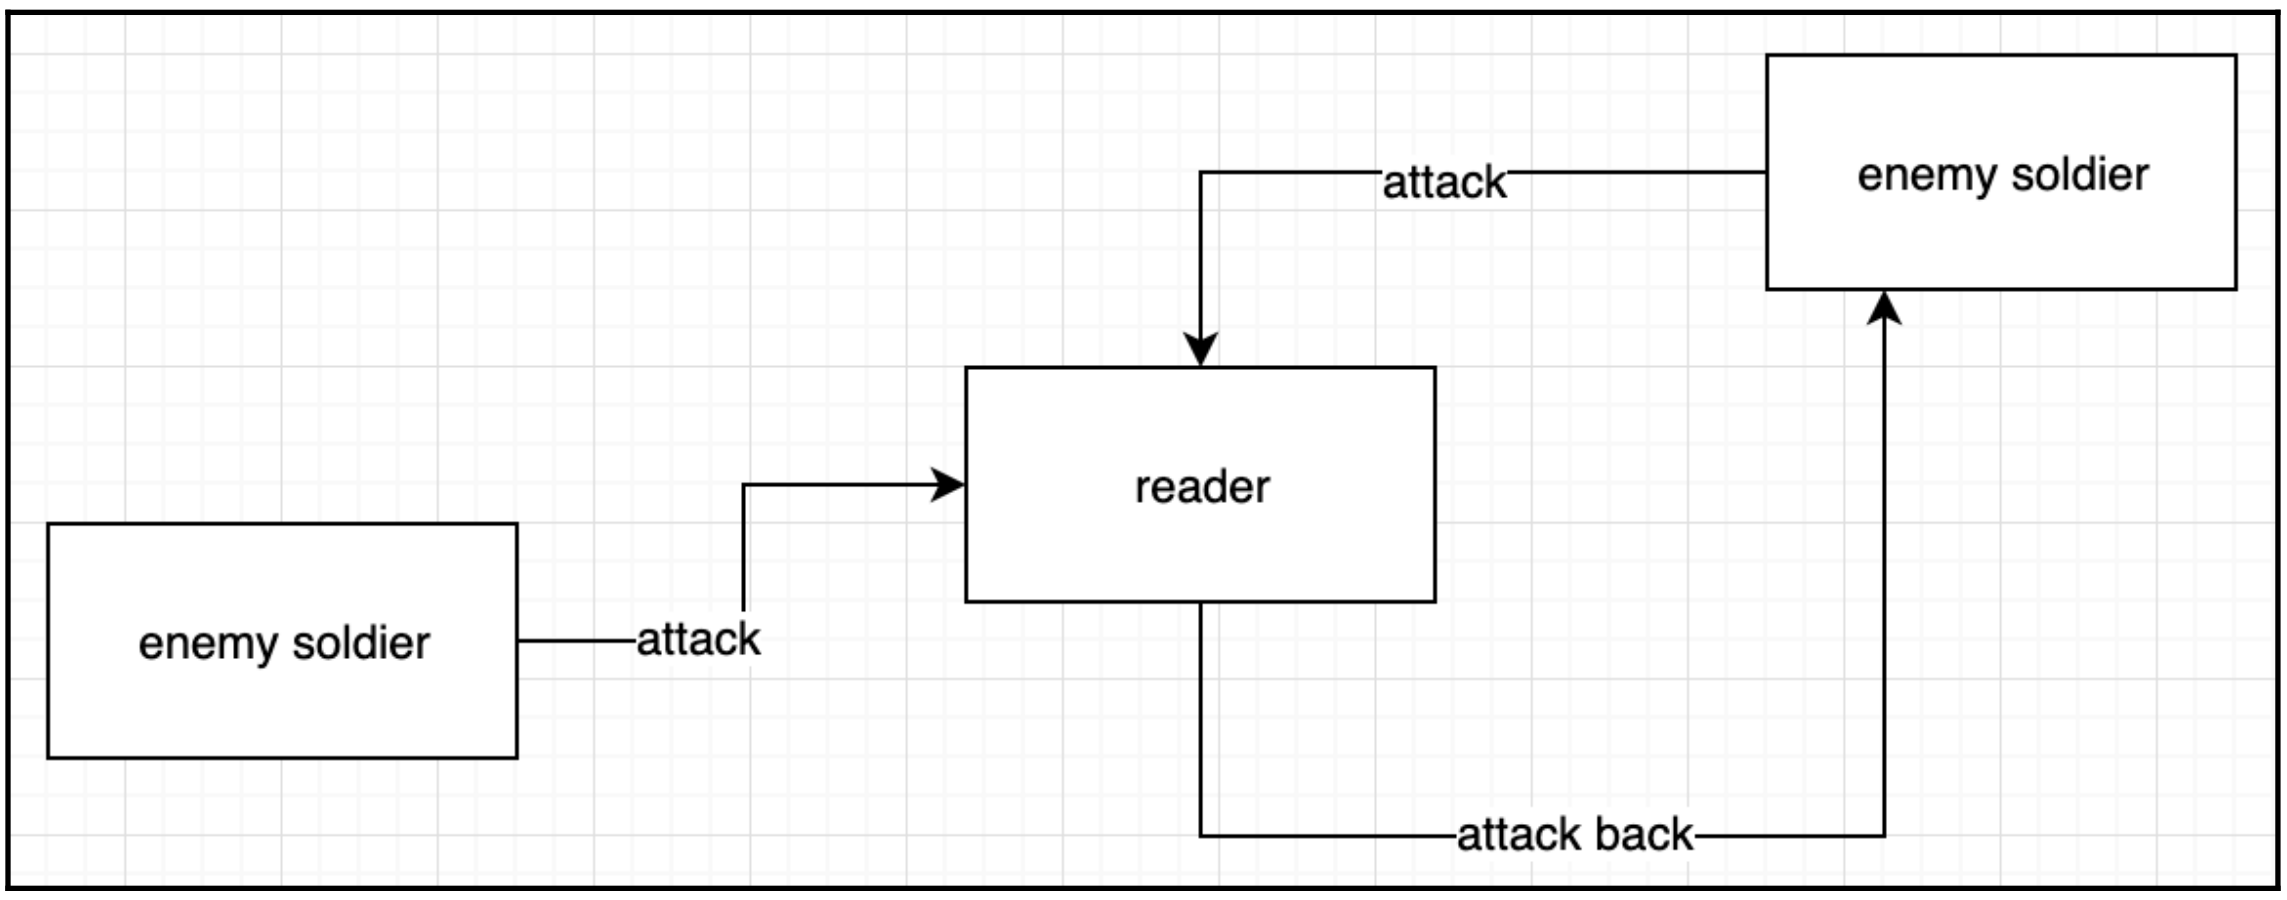
\includegraphics[width=1.0\textwidth]{content/Section-2/Chapter-11/2}
\end{center}

更多的互动发生在游戏中。游戏中有两组,其中一组由玩家控制。另一个是由电脑控制。这意味着作为游戏设计师必须定义敌人。游戏将自动创建读者,并分配给他们创建图书馆、兵营和房屋的任务。每个士兵都应该承担保卫建筑物和读者(人民)的责任。有时,士兵们应该聚在一起,执行攻击任务。 \par
我们将设计一个平台,让玩家创建一个帝国,而游戏也应该创造敌人来完善游戏。玩家将经常面临敌人的攻击,敌人将通过建造更多建筑和生产更多单位而进化。总的来说,我们可以用下图来描述交互: \par

\begin{center}
	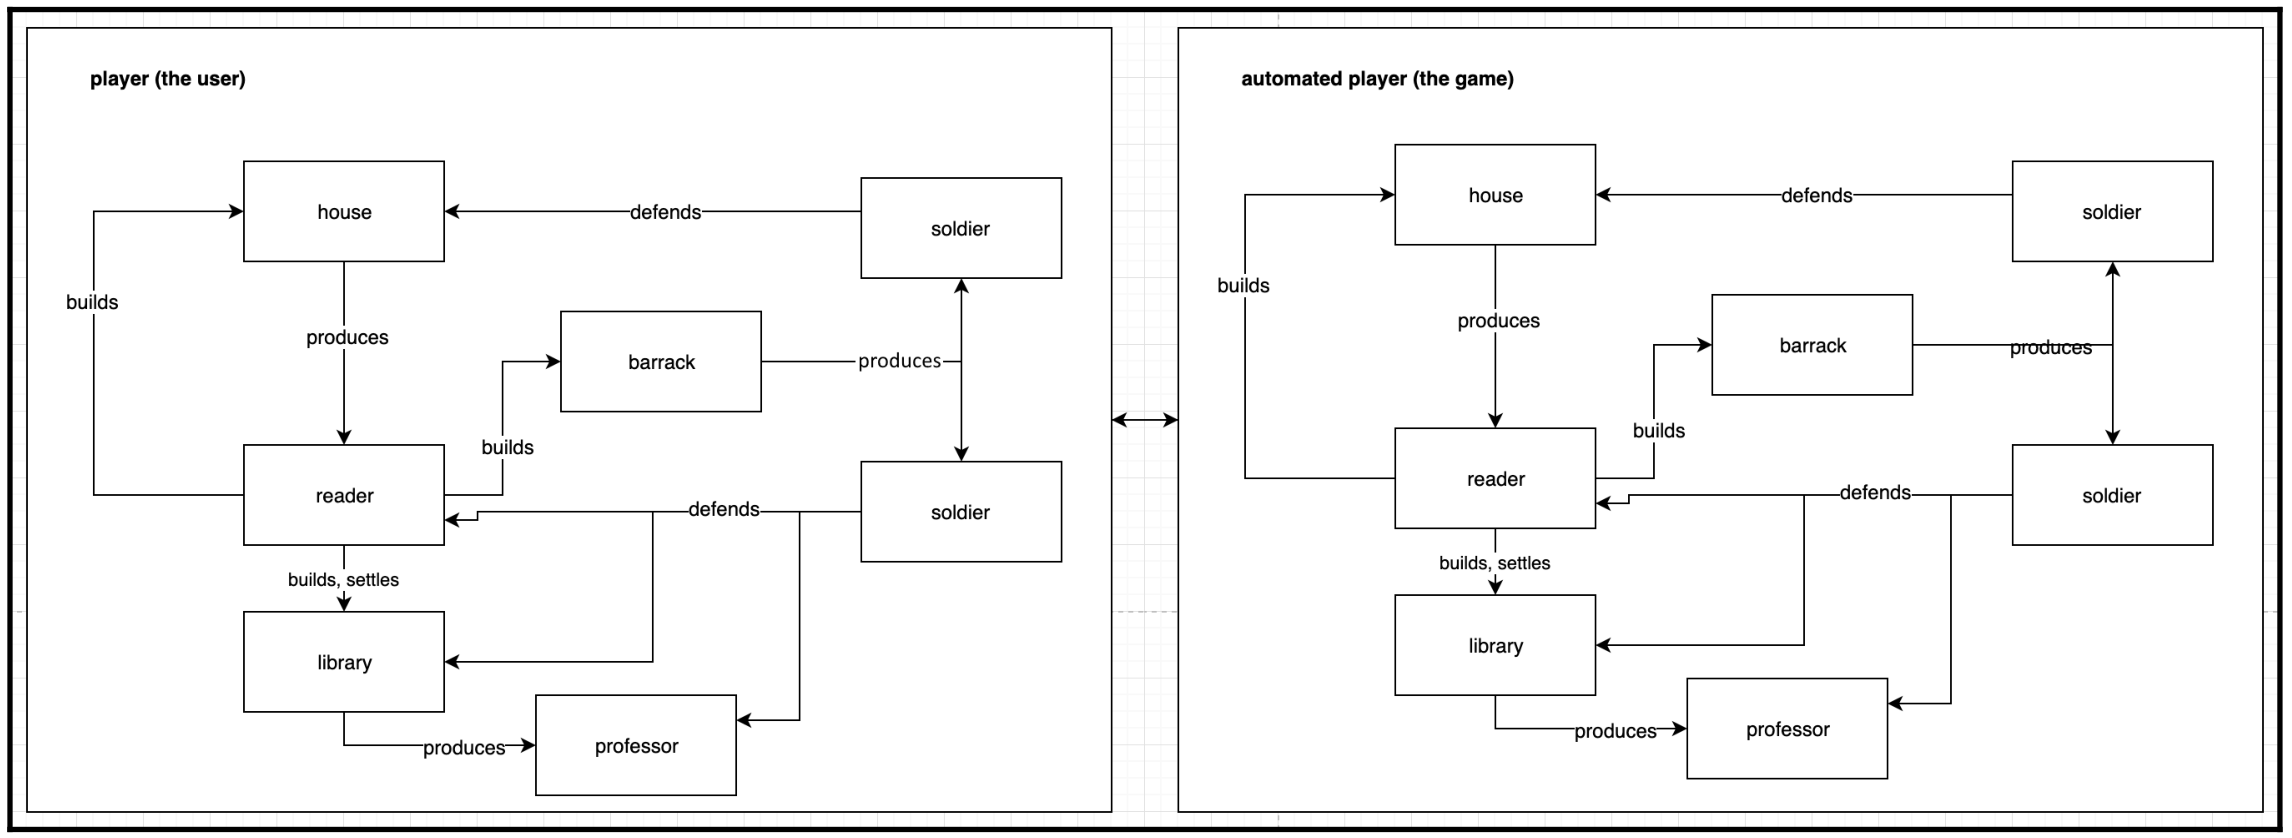
\includegraphics[width=1.0\textwidth]{content/Section-2/Chapter-11/3}
\end{center}

我们将在设计游戏时参考上述图表。 \par

\noindent\textbf{}\ \par
\textbf{设计游戏} \ \par
虽然游戏并不是一款典型的软件,但它的设计却与常规应用设计并无太大区别。我们将从主要实体开始,并将它们进一步分解为类的关系。 \par
在前一节中,我们讨论了游戏组件及其交互作用。我们根据项目开发生命周期进行了需求分析和收集。现在,我们开始设计游戏。 \par

\noindent\textbf{}\ \par
\textbf{设计角色} \ \par
下面的类图代表了一个读者: \par

\begin{center}
	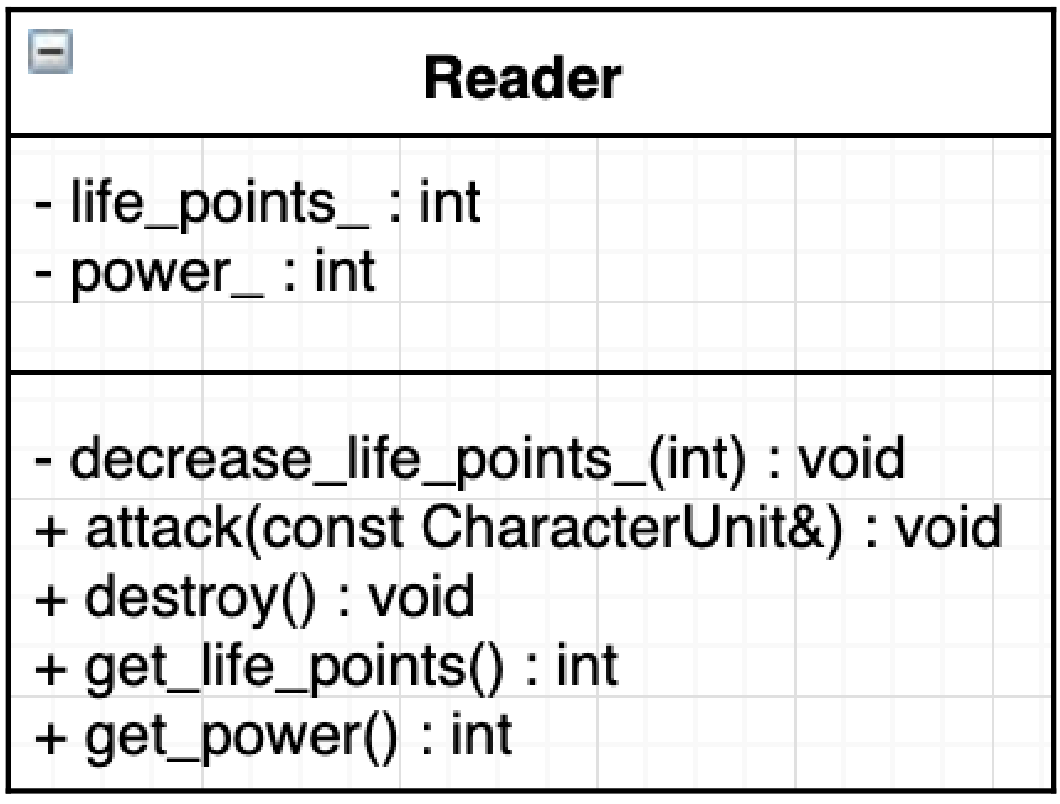
\includegraphics[width=0.6\textwidth]{content/Section-2/Chapter-11/4}
\end{center}

当我们浏览其他角色单位时,我们将为每个角色单位想出一个基类。每个特定的单元将从这个基类继承,并添加特定的属性(如果有的话)。以下是角色单位的完整类图: \par

\begin{center}
	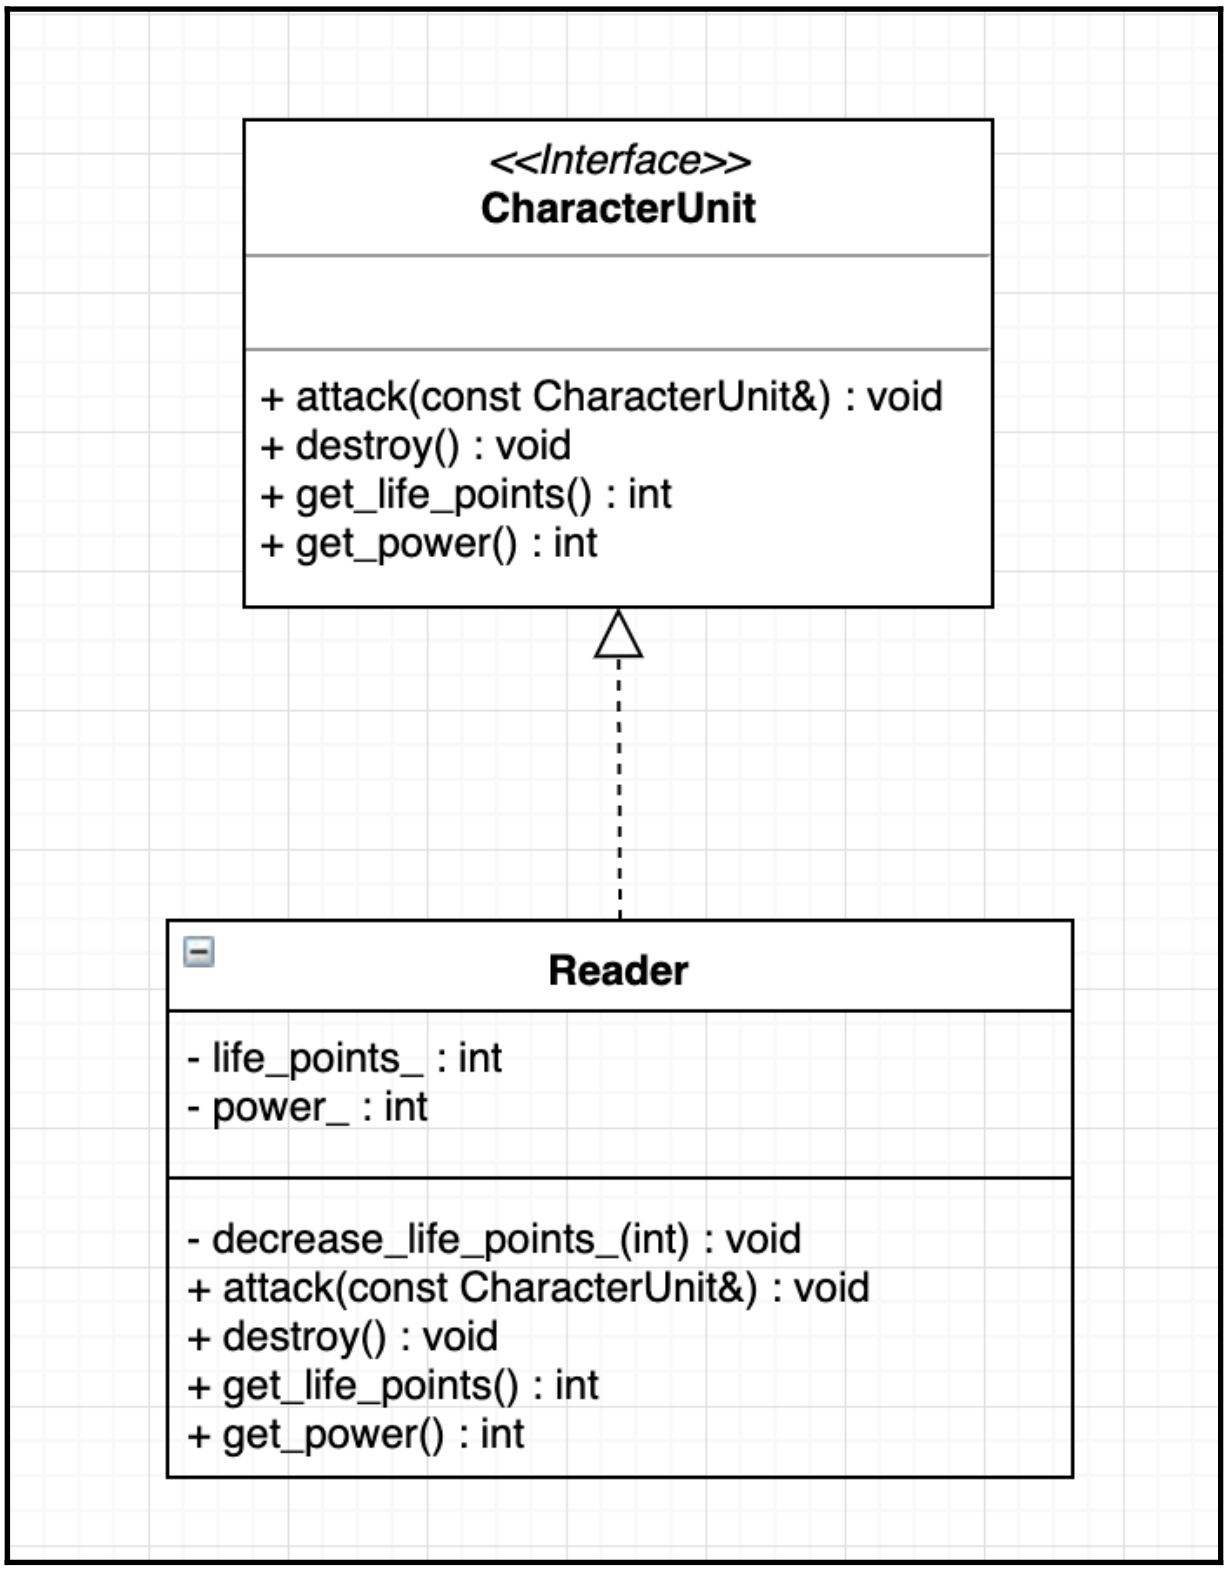
\includegraphics[width=0.6\textwidth]{content/Section-2/Chapter-11/5}
\end{center}

请注意基类——它是一个接口,而不是一个常规类。它定义了在派生类中实现的纯虚函数。以下是CharacterUnit接口在代码中的声明: \par

\begin{lstlisting}[caption={}]
class CharacterUnit
{
public:
	virtual void attack(const CharacterUnit&) = 0;
	virtual void destroy() = 0;
	virtual int get_power() const = 0;
	virtual int get_life_points() const = 0;
};
\end{lstlisting}

attack()会降低角色的生命值,destroy()则会摧毁角色。摧毁不仅意味着将角色从场景中移除,还意味着停止该单位正在进行的所有互动(如建造建筑、自卫等等)。 \par
派生类提供了CharacterUnit接口类的纯虚函数的实现。让我们来看看Reader字符单元的代码: \par

\begin{lstlisting}[caption={}]
class Reader : public CharacterUnit
{
public:
	Reader();
	Reader(const Reader&) = delete;
	Reader& operator=(const Reader&) = delete;
	
public:
	void attack(const CharacterUnit& attacker) override {
		decrease_life_points_by_(attacker.get_power());
	}

	void destroy() override {
		// we will leave this empty for now
	}

	int get_life_points() const override {
		return life_points_;
	}

	int get_power() const override {
		return power_;
	}

private:
	void decrease_life_points_(int num) {
		life_points_ -= num;
		if (life_points_ <= 0) {
			destroy();
		}
	}

private:
	int life_points_;
	int power_;
};
\end{lstlisting}

现在,我们可以通过以下任何一种方式声明Reader: \par

\begin{lstlisting}[caption={}]
Reader reader;
Reader* pr = new Reader();
CharacterUnit* cu = new Reader();
\end{lstlisting}

主要通过基接口类来引用角色单位。 \par

\hspace*{\fill} \\ %插入空行

\includegraphics[width=0.05\textwidth]{images/tip}
请注意复制构造函数和赋值操作符。我们故意把它们标记为删除,因为我们不想通过复制其他单位来创建单位。我们将为该行为使用原型模式。这将在后面讨论。 \par
\noindent\textbf{}\ \par

我们应该为不同类型的单位做同样的事情的场景中,拥有CharacterUnit接口非常重要,例如:我们必须计算两名士兵、一名读者和一名教授对一座建筑造成的全部损害。我们不必保留三个不同的引用来引用三种不同类型的单元,而是将它们都称为CharacterUnits。方法如下: \par

\begin{lstlisting}[caption={}]
int calculate_damage(const std::vector<CharacterUnit*>& units)
{
	return std::reduce(units.begin(), units.end(), 0,
		[](CharacterUnit& u1, CharacterUnit& u2) {
			return u1.get_power() + u2.get_power();
		}
	);
}
\end{lstlisting}

calculate\underline{ }damage()函数对单元类型进行抽象,它不关心读者或士兵。它只调用CharacterUnit接口的get\underline{ }Ppower()方法,该方法保证特定对象的实现。\par
我们将更新角色单位类,让我们继续为建筑设计类。 \par

\noindent\textbf{}\ \par
\textbf{设计建筑} \ \par
建筑类型与角色单位的接口相似。例如,可以定义建筑的类: \par

\begin{lstlisting}[caption={}]
class House
{
public:
	House();
	// copying will be covered by a Prototype
	House(const House&) = delete;
	House& operator=(const House&) = delete;
	
public:
	void attack(const CharacterUnit&);
	void destroy();
	void build(const CharacterUnit&);
	// ...
	
private:
	int life_points_;
	int capacity_;
	std::chrono::duration<int> construction_duration_;
};
\end{lstlisting}

我们使用std::chrono::duration来统计房屋建造的时长,它在<chrono>头文件中定义为一个刻度数和一个刻度周期,其中刻度周期是从一个刻度到下一个刻度的秒数。 \par
House类需要更多的细节,需要为所有的建筑提供一个基接口(甚至是一个抽象类)。在本章中描述的建筑都有相同的行为。建筑接口如下: \par

\begin{lstlisting}[caption={}]
class IBuilding
{
public:
	virtual void attack(const CharacterUnit&) = 0;
	virtual void destroy() = 0;
	virtual void build(CharacterUnit*) = 0;
	virtual int get_life_points() const = 0;
};
\end{lstlisting}

注意建筑物前面的I前缀。许多开发人员建议为接口类使用前缀或后缀,以提高可读性。例如,Building可能被命名为IBuilding或BuildingInterface。我们将对前面描述的CharacterUnit使用相同的命名技术。 \par
House、Barrack和Library类实现了IBuilding接口,并且必须提供纯虚方法的实现。例如,Barrack类如下所示: \par

\begin{lstlisting}[caption={}]
class Barrack : public IBuilding
{
public:
	void attack(const ICharacterUnit& attacker) override {
		decrease_life_points_(attacker.get_power());
	}

	void destroy() override {
		// we will leave this empty for now
	}

	void build(ICharacterUnit* builder) override {
		// construction of the building
	}

	int get_life_points() const override {
		return life_points_;
	}

private:
	int life_points_;
	int capacity_;
	std::chrono::duration<int> construction_duration_;
};
\end{lstlisting}

让我们更详细地讨论构建时长的实现,std::chrono::duration可以告诉我们构建花费的时间。另外,请注意,类的最终设计可能在本章的行文过程中发生变化。现在,让我们看看如何让游戏的组件彼此互动。 \par

\noindent\textbf{}\ \par
\textbf{设计游戏控制器} \ \par
为角色单位和建筑设计类型只是设计游戏的第一步。游戏中最重要的组件间的互动。我们需要仔细分析和设计案例,比如:两个或两个以上的读者建造一座建筑。我们已经介绍了建筑的建造时间,但我们没有考虑到一个建筑可能由多个读者建造(可以建造建筑的角色单位)。 \par
两个读者建一座大楼的速度应该比一个读者建的快两倍。如果另一个读者加入了,我们应该重新计算持续时间。然而,我们应该限制能建造同一建筑的读者数量。 \par
如果读者被敌人攻击,这会打断读者建造,他们会进行自卫。当读者停止在建筑上工作时,我们应该重新计算施工时间。当角色受到攻击时,它应该反击来保护自己。每次命中都会减少角色的生命值。一个角色可能同时受到多个敌人角色的攻击。这将更快地降低他们的生命值。 \par
建筑有一个计时器,它会周期性地产生角色。设计最重要的是游戏动态,也就是循环。在每个特定的时间框架,游戏中都会发生一些事情。这可能是敌人士兵靠近,角色单位建造东西,或其他任何东西。一个操作的执行与另一个不相关的操作的完成没有严格的联系。这意味着建筑的建造与角色的创造同时发生。与大多数应用程序不同,游戏应该保持移动,即使用户不提供任何输入。如果玩家未能执行某个行动,游戏也不会停止。角色单位可能会等待一个命令,但是建筑会继续工作——产生新的角色。同样地,敌人玩家(自动玩家)也会为胜利不停的奋斗。 \par

\noindent\textbf{}\ \par
\textbf{并发行为} \ \par
游戏中的许多行动是同时发生的。就像我们之前所讨论的,建筑的建造不应该因为未参与建造的单位或受到敌人的攻击而停止。这意味着我们应该为游戏中的许多对象设计并发行为。 \par
C++中实现并发的最佳方法是使用线程。我们可以重新设计单位和建筑,以便它们在基类中有可重写的动作,该动作将在单独的线程中执行。让我们重新设计IBuilding,使它成为一个抽象类,它有一个额外的run()虚函数: \par

\begin{lstlisting}[caption={}]
class Building
{
public:
	virtual void attack(const ICharacterUnit&) = 0;
	virtual void destroy() = 0;
	virtual void build(ICharacterUnit*) = 0;
	virtual int get_life_points() const = 0;
	
public:
	void run() {
		std::jthread{Building::background_action_, this};
	}

private:
	virtual void background_action_() {
		// no or default implementation in the base class
	}
};
\end{lstlisting}

注意background\underline{ }action\underline{ }()函数,它是私有的,但却是虚的,我们可以在派生类中重写它。run()函数不是虚函数,它在线程中运行私有实现。派生类可能会提供background\underline{ }action\underline{ }()的实现。当一个单元来建造建筑时,就会调用build()虚函数。build()函数将计算构造时间的工作委托给run()函数。 \par

\noindent\textbf{}\ \par
\textbf{游戏事件循环} \ \par
解决这个问题最简单的方法是定义一个事件循环。事件循环如下所示: \par

\begin{lstlisting}[caption={}]
while (true)
{
	processUserActions();
	updateGame();
}
\end{lstlisting}

即使用户(玩家)没有采取任何行动,游戏仍然通过调用updateGame()函数继续运行。请注意,前面的代码只是对事件循环的介绍,它会无限循环并在每次迭代中处理和更新游戏。 \par
每次循环迭代都会推进游戏状态。如果用户操作处理需要很长时间,它可能会阻塞循环,游戏会暂停一会儿。我们通常以每秒帧数(FPS)来衡量游戏速度。值越高,游戏就越流畅。 \par
我们需要设计在游戏过程中持续运行的游戏循环。重要的是要将其设计成用户操作处理不会阻塞循环的方式。 \par
游戏循环负责处理游戏中发生的一切,包括AI。关于AI,指的是之前讨论过的电脑玩家。除此之外,游戏循环还会处理角色的行动,并相应地更新游戏状态。 \par
在深入研究游戏循环设计之前,让我们先了解一些能够帮助我们完成这一复杂任务的设计模式。毕竟,游戏循环是另一种设计模式! \par

\noindent\textbf{}\ \par
\textbf{使用设计模式} \ \par
使用面向对象编程(OOP)范式设计游戏是很香的,游戏代表的是物体之间紧密互动的组合。在我们的策略游戏中,我们的建筑由单位建造。单位防御敌人单位等。这种内部交流导致了复杂性的增长。随着项目的发展和更多特性的增加,维护将变得更加困难。很明显,设计是建筑项目中最重要的部分之一。合并设计模式将大大改善设计过程和项目支持。 \par
让我们来看看一些在游戏开发中有用的设计模式。我们将从经典模式开始,然后讨论更多特定于游戏的模式。 \par

\noindent\textbf{}\ \par
\textbf{命令模式} \ \par
开发人员将设计模式分为创建的、结构的和行为的三种类别。命令模式是一种行为设计模式。行为设计模式主要关注在对象之间的通信中提供灵活性。在此上下文中,命令模式将操作封装在一个对象中,该对象包含必要的信息以及操作本身。这样,命令模式的行为就像一个智能函数。在C++中实现它的最简单方法是重载类的函数操作(),如下所示: \par

\begin{lstlisting}[caption={}]
class Command
{
	public:
	void operator()() { std::cout << "I'm a smart function!"; }
};
\end{lstlisting}

带有重载函数操作符()的类有时称为仿函数。以上代码与下面的常规函数声明相同: \par

\begin{lstlisting}[caption={}]
void myFunction() { std::cout << "I'm not so smart!"; }
\end{lstlisting}

调用常规函数和Command类的对象看起来类似,如下所示: \par

\begin{lstlisting}[caption={}]
myFunction();
Command myCommand;
myCommand();
\end{lstlisting}

当我们需要为函数使用状态时,这两者之间的区别很明显。为了存储常规函数的状态,我们使用静态变量。为了在对象中存储状态,我们使用对象本身。下面是如何跟踪重载函数操作符的调用次数: \par

\begin{lstlisting}[caption={}]
class Command
{
public:
	Command() : called_(0) {}
	
	void operator()() {
		++called_;
		std::cout << "I'm a smart function." << std::endl;
		std::cout << "I've been called" << called_ << " times." << std::endl;
	}
private:
	int called_;
};
\end{lstlisting}

调用的数量对于命令类的每个实例是唯一的。下面的代码声明了两个Command实例,并分别调用它们两次和三次: \par

\begin{lstlisting}[caption={}]
Command c1;
Command c2;
c1();
c1();
c2();
c2();
c2();
// at this point, c1.called_ equals 2, c2.called_ equals 3
\end{lstlisting}

现在,让我们尝试将这个模式应用到我们的策略游戏中。游戏的最终版本有一个图形界面,允许用户使用各种按钮和鼠标点击来控制游戏。例如,要让一个角色单位建造一座房子,而不是一个兵营,我们应该在游戏面板上选择相应的图标。让我们想象一个带有游戏地图和一些控制游戏动态的按钮的游戏面板。 \par
游戏向玩家提供以下命令: \par

\begin{itemize}
	\item 将角色单位从A点移动到B点
	\item 攻击敌人
	\item 建造建筑
	\item 攻击建筑
\end{itemize}

游戏命令的设计如下: \par

\begin{center}
	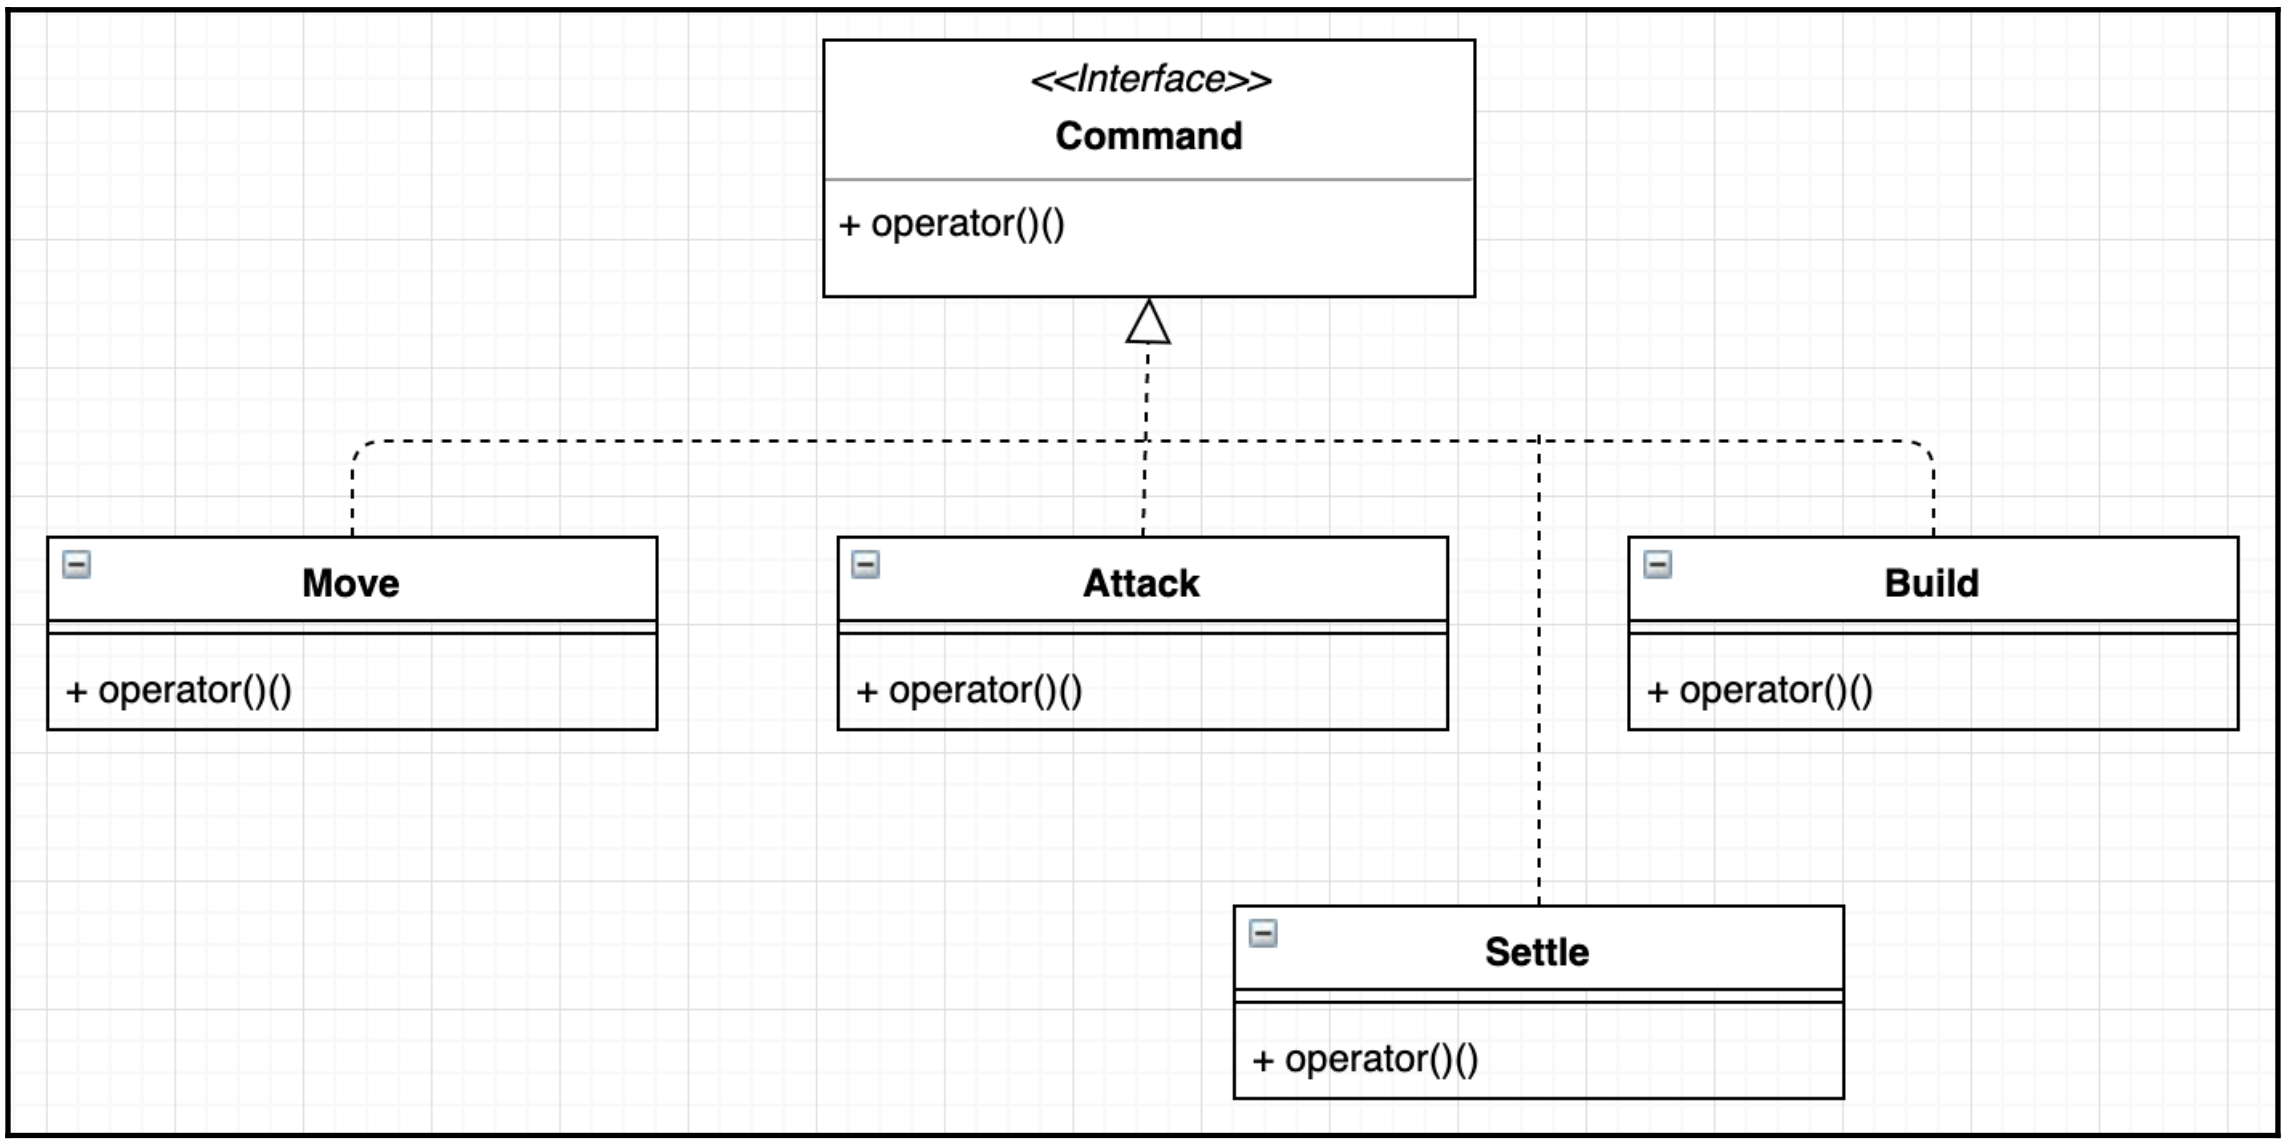
\includegraphics[width=1.0\textwidth]{content/Section-2/Chapter-11/6}
\end{center}

每个类都封装了操作逻辑。客户端代码与处理操作无关。它使用命令指针进行操作,每个命令指针都指向具体的命令(如前面的图像所示)。注意,我们只描述了玩家将执行的命令。游戏本身使用命令在模块之间进行通信,自动命令的例子包括Run、Defend、Die和Create。下面是一个更广泛的图表,展示了游戏中的命令: \par

\begin{center}
	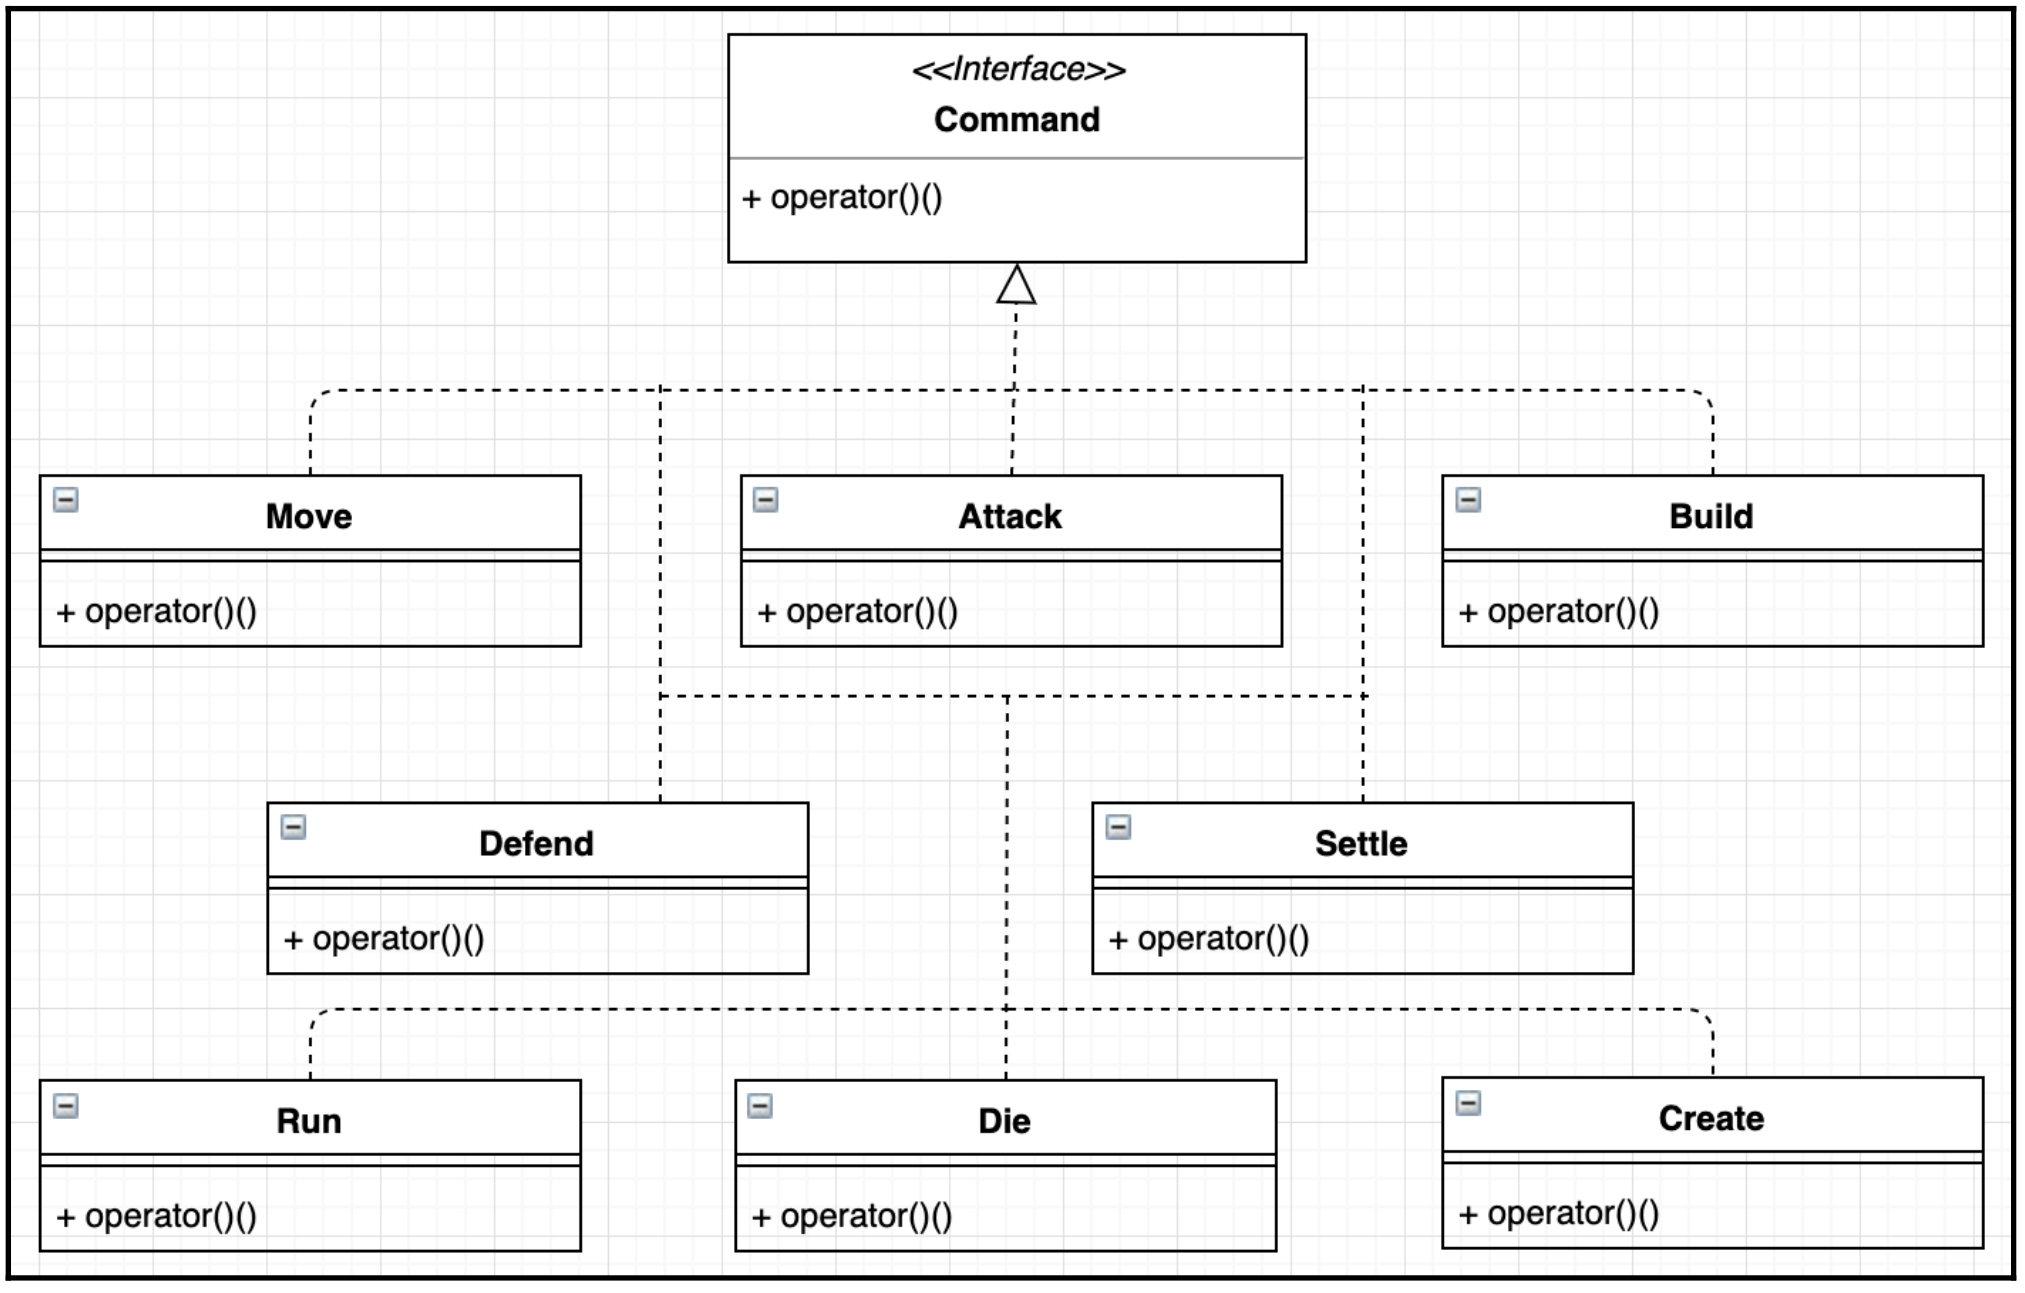
\includegraphics[width=1.0\textwidth]{content/Section-2/Chapter-11/7}
\end{center}

上述命令执行游戏玩法中出现的任何事件。为了监听这些事件,我们应该考虑使用观察者模式。 \par

\noindent\textbf{}\ \par
\textbf{观察者模式} \ \par
观察者模式是一种体系结构机制,允许我们关注对象状态更改,我们观察物体的变化。观察者模式也是一种行为设计模式。 \par
大多数策略游戏都包含资源的概念。可能是石材、金币、木材等,例如:在建造一座建筑时,玩家需要花费20个木材,40个石材和10个金币。最终,玩家将耗尽资源并需要收集这些资源。这个玩家创造了更多的角色单位,并让他们收集资源——几乎就像在现实生活一样。 \par
现在,我们假设游戏中也有类似的资源收集。当玩家让单位收集资源时,他们应该在每次收集到固定数量的资源时通知我们。玩家是资源收集事件的关注者。 \par
建筑也是如此。建筑物产生一个角色-玩家会收到通知。一个角色单位完成建筑建造-玩家会收到通知。我们更新玩家仪表板以保持玩家的游戏状态更新,玩家在玩游戏时可以了解拥有多少资源、多少单位和多少建筑。 \par
观察者涉及到实现一个类,该类存储其关注者并在事件上调用指定的函数。它由两个实体组成:关注者和执行者。如下图所示,用户数量不限于1个: \par

\begin{center}
	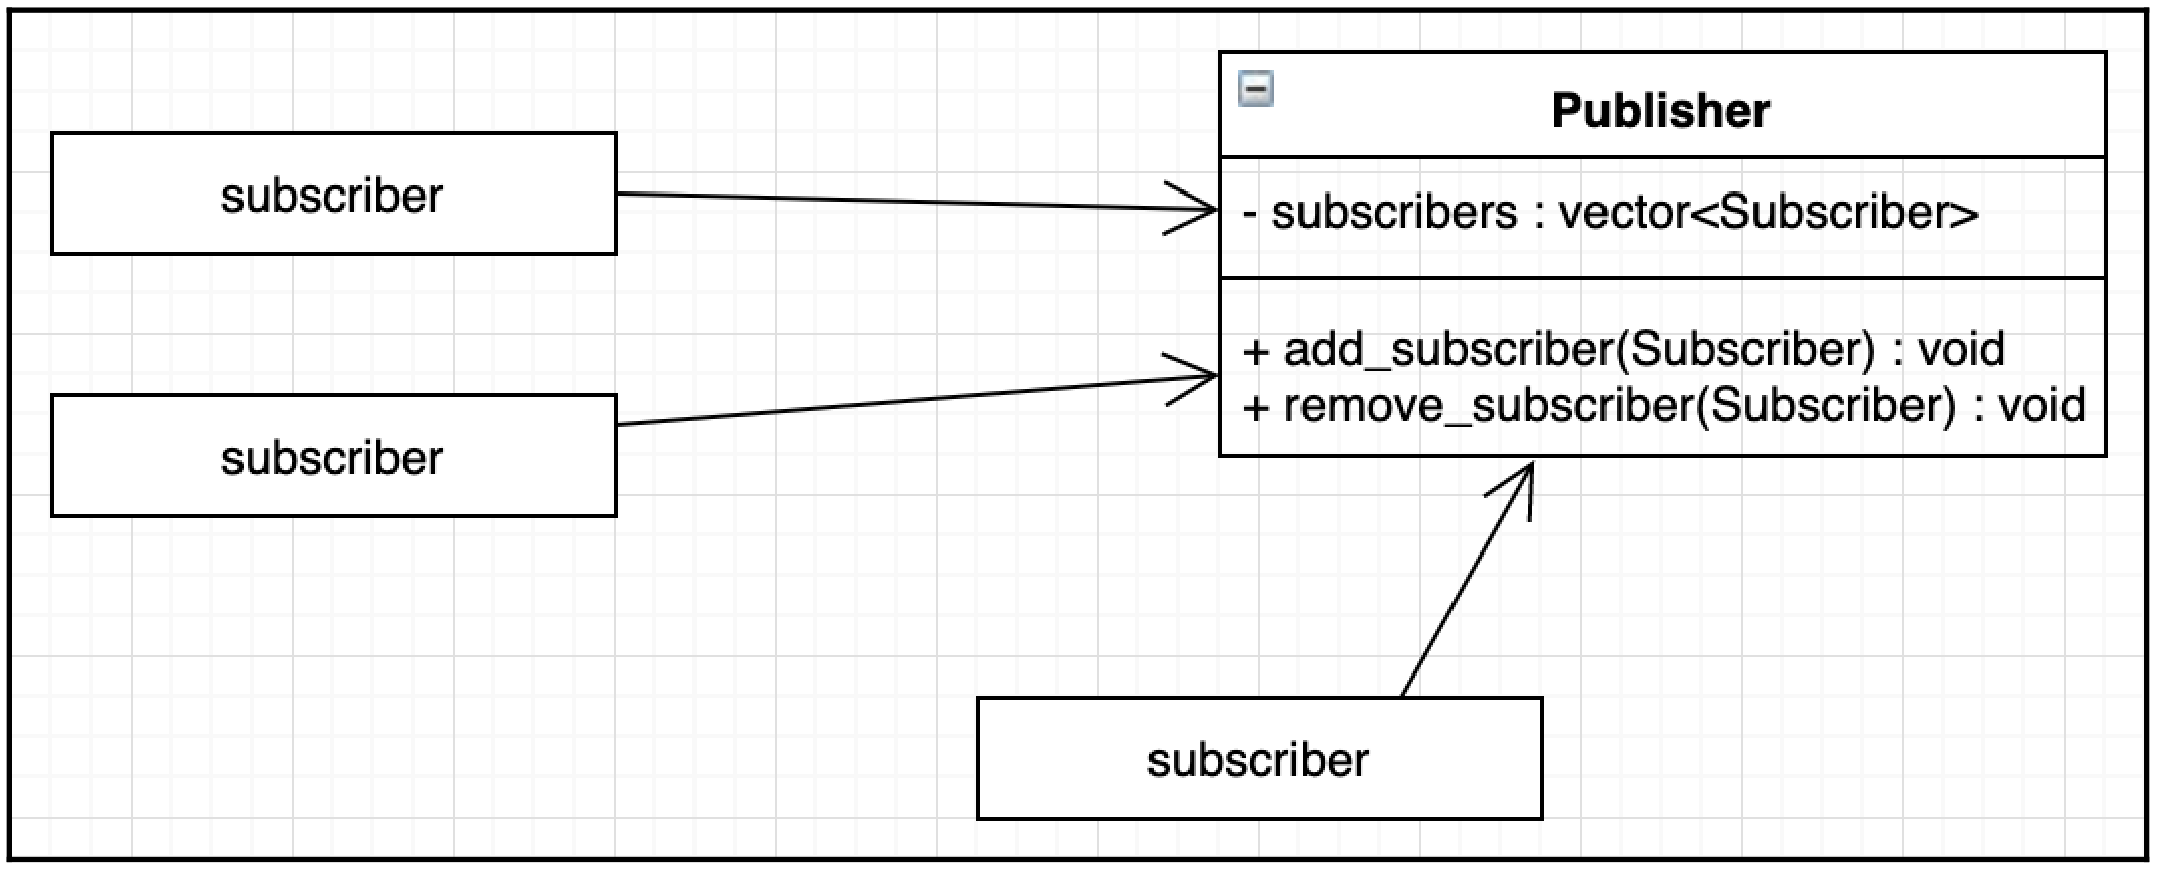
\includegraphics[width=1.0\textwidth]{content/Section-2/Chapter-11/8}
\end{center}

例如,当一个角色单位去建造一座建筑时,它会不断的去建造,除非被阻止。造成这种情况的原因有很多: \par

\begin{itemize}
	\item 玩家决定取消建造建筑的过程。
	\item 角色单位必须防御敌人的攻击,并暂停建造过程。
	\item 建筑已经完成,所以角色单位停止了工作。
\end{itemize}

玩家还希望在建筑完成时得到通知,因为他们可能计划在完成建筑后让角色单位执行其他任务。我们可以设计构建流程,使其在事件完成时通知其侦听器(关注者)。下面的类图还涉及到一个操作接口。将其视为命令模式的实现: \par

\begin{center}
	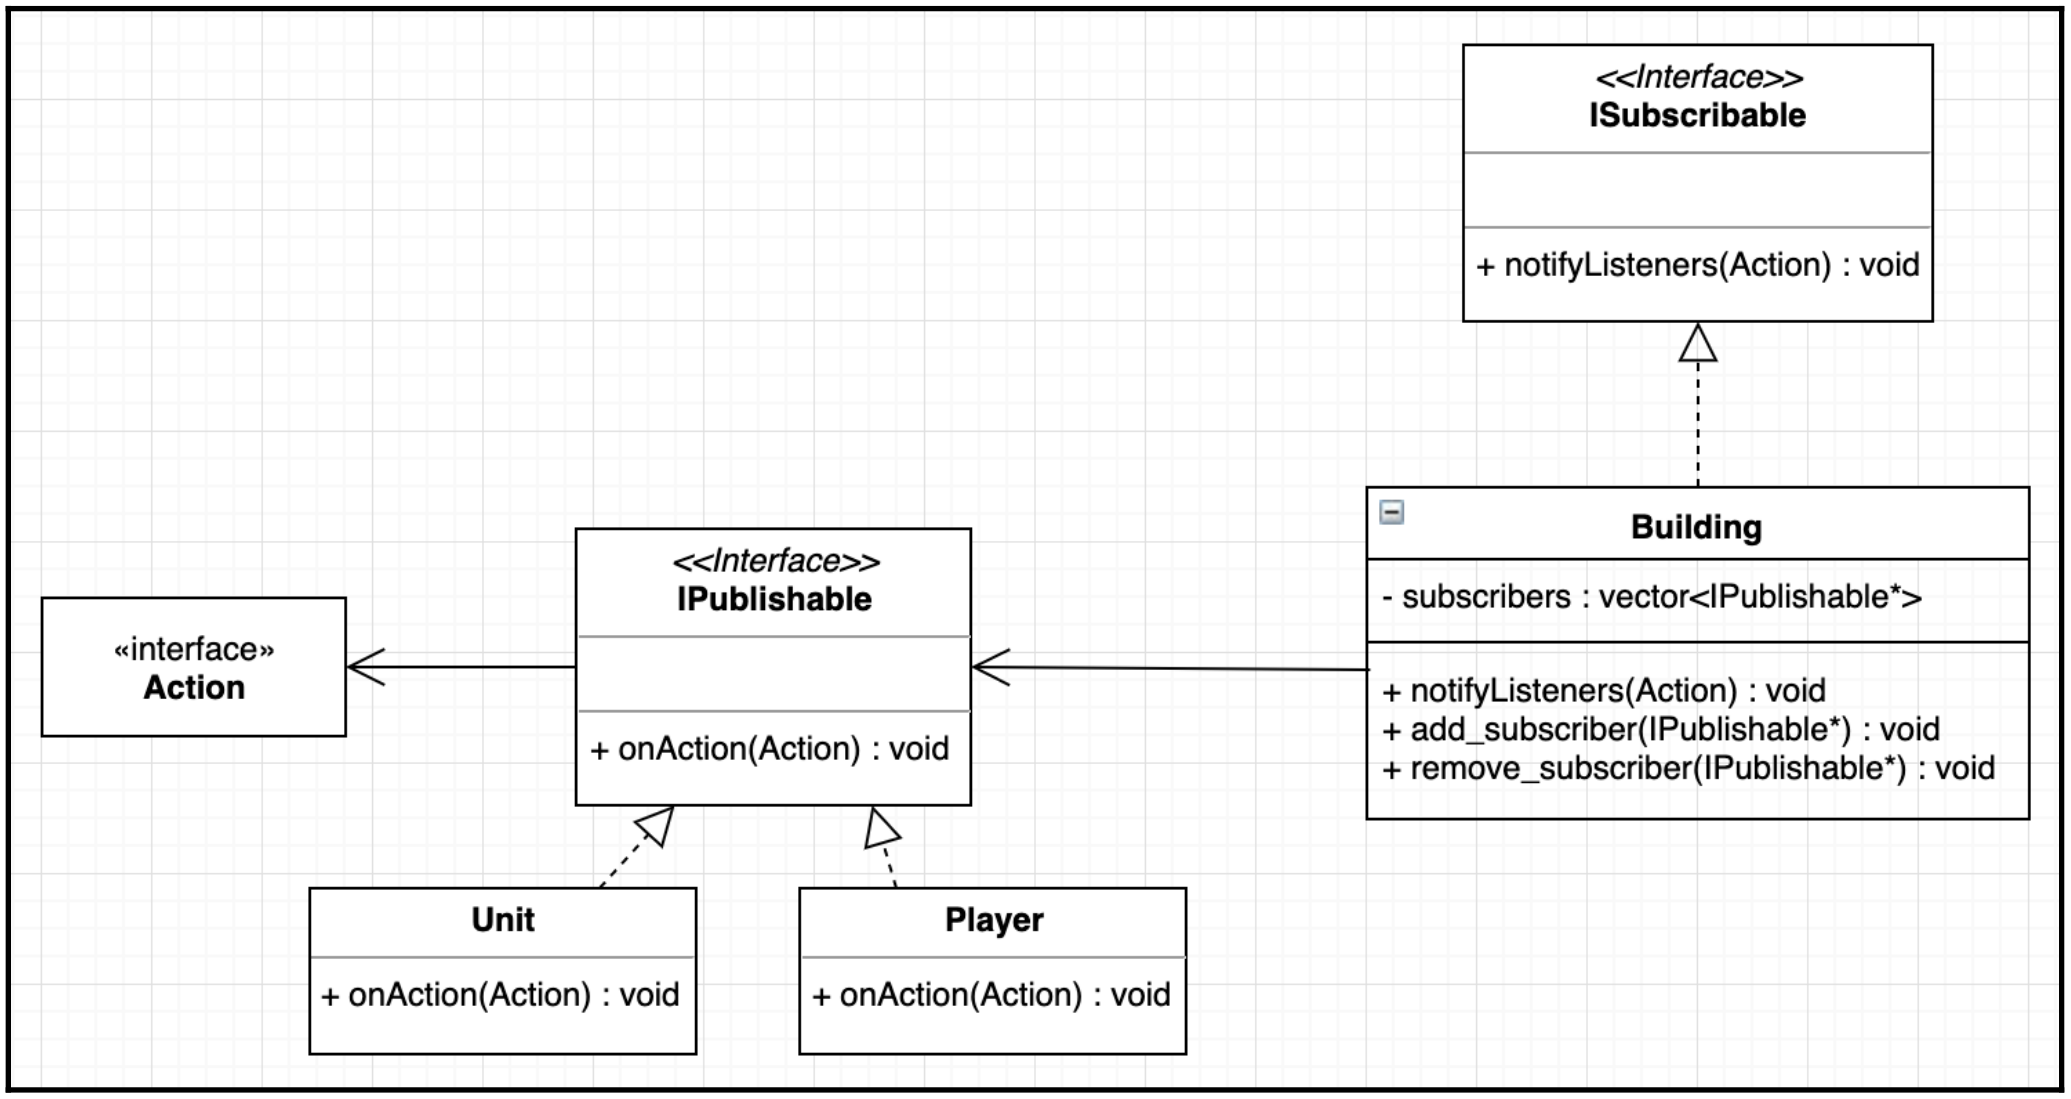
\includegraphics[width=1.0\textwidth]{content/Section-2/Chapter-11/9}
\end{center}

针对观察者开发类会让我们意识到,游戏中几乎所有的实体都是关注者、执行者或两者兼有。如果您遇到类似的场景,您可以考虑使用中介——另一种行为模式。对象通过中介对象相互通信。触发事件的对象可以让中介知道该事件。然后,中介将消息传递给“订阅”到对象状态的任何相关对象。下图是中介集成的简化版本: \par

\begin{center}
	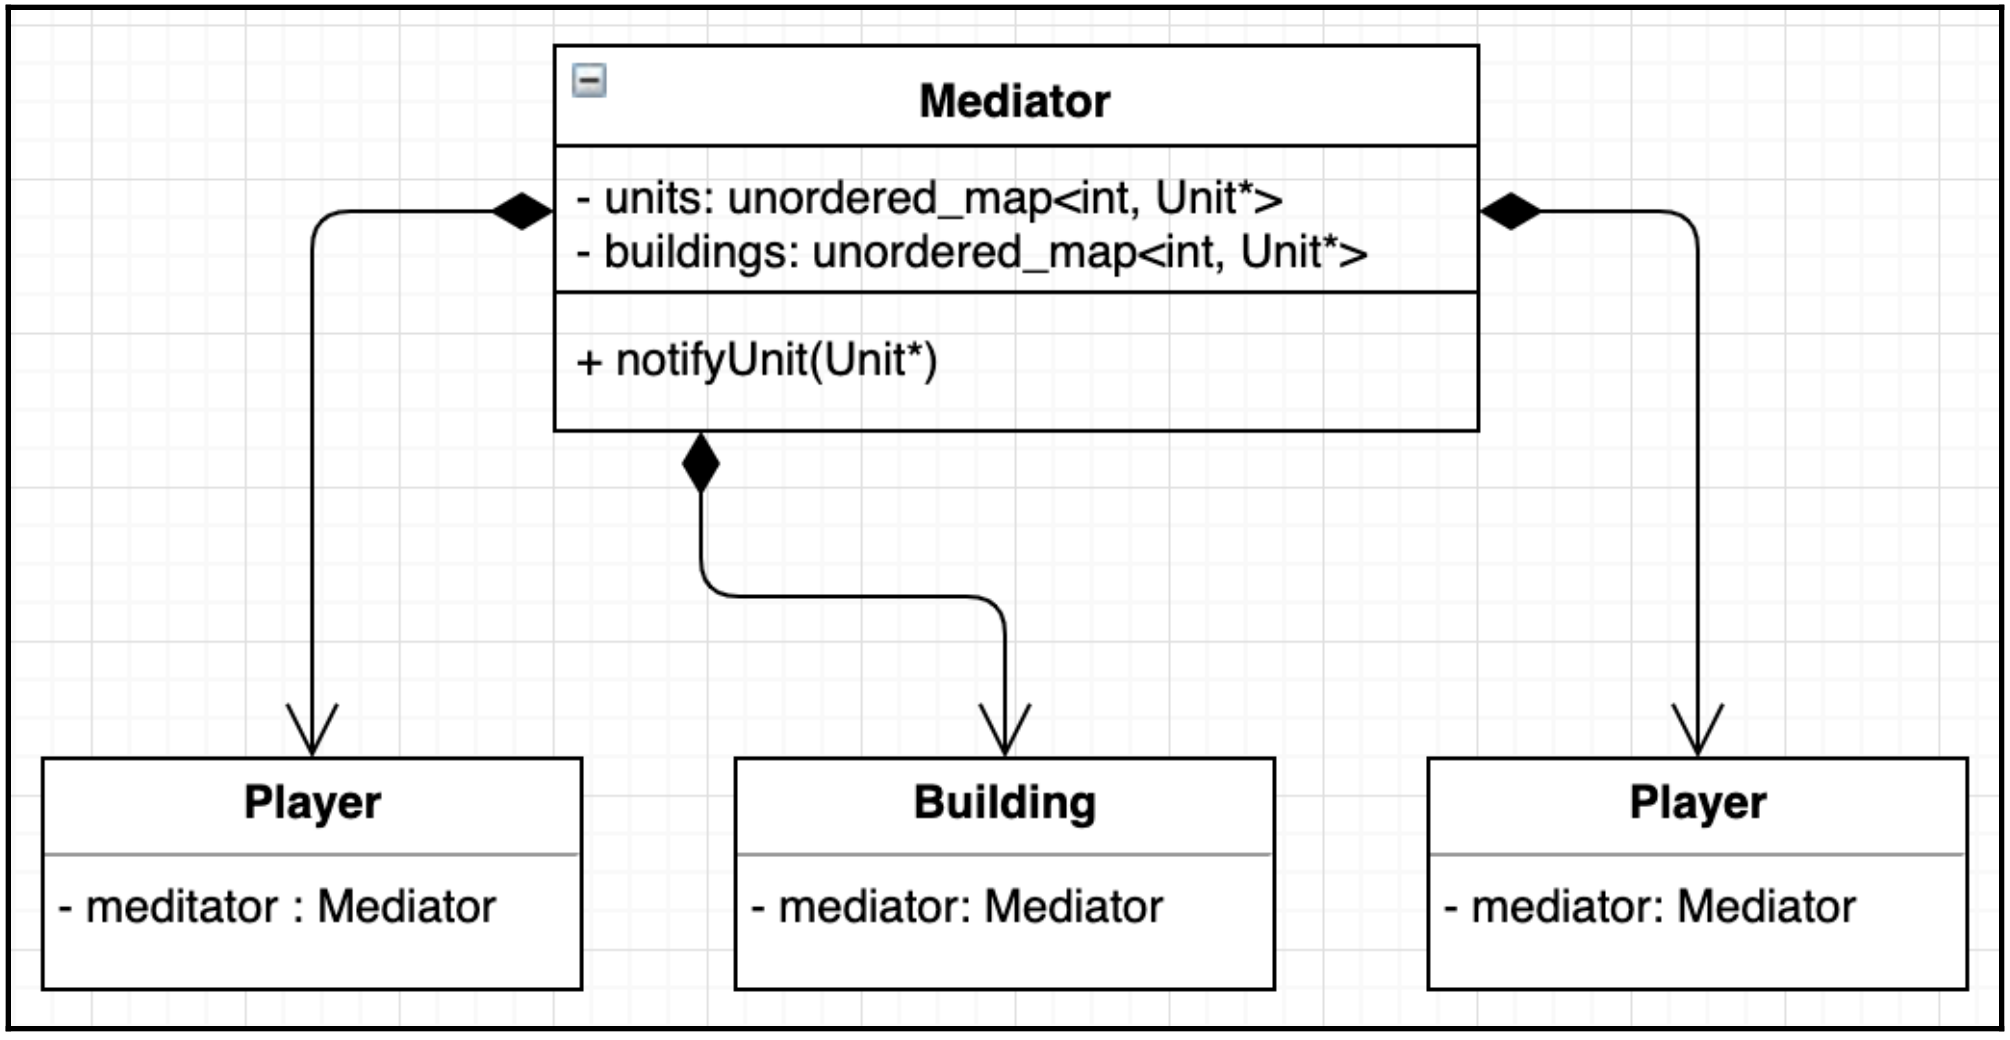
\includegraphics[width=1.0\textwidth]{content/Section-2/Chapter-11/10}
\end{center}

每个对象都包含一个中介,用于将更改通知关注者。中介对象通常包含所有相互通信的对象。对于事件,每个对象通过中介通知相关方,例如:当构建构建完成时,会触发中介,中介会通知所有关注方。要接收这些通知,每个对象都应该事先关注中介。 \par

\noindent\textbf{}\ \par
\textbf{享元模式} \ \par
享元是一种结构设计模式。结构模式负责将对象和类组装成更大、更灵活的结构。享元允许我们通过共享对象的公共部分来缓存对象。 \par
在策略游戏中,我们要处理许多呈现在屏幕上的对象。游戏过程中,对象的数量会增加。玩家玩游戏的时间越长,创造的角色单位和建筑就越多(敌人也是如此)。游戏中的每个单位代表一个包含数据的独立对象。字符单元至少占用16个字节的内存(对于它的两个整数数据成员和虚拟表指针)。 \par
当我们为了在屏幕上呈现单位而添加额外字段时,情况就变得更糟了。例如,它们的高度、宽度和精灵(代表渲染单元的图像)。除了角色单位之外,游戏还应该添加一些辅助道具,例如:树、石头等装饰性道具,以提升用户体验。某种程度上,我们在屏幕上渲染了大量对象,每个对象几乎代表相同的对象,但它们的状态有微小的差异。享元模式在这里起到了很大的作用。对于角色单位,它的高度、宽度和精灵在所有单位中存储了几乎相同的数据。 \par
享元模式建议将一个重物体分解成两个: \par

\begin{itemize}
	\item 一个不可变的对象,它为相同类型的每个对象包含相同的数据
	\item 一个可变对象,将自己与其他对象区分开来
\end{itemize}

例如,一个移动的角色单位有它自己的高度、长度和精灵,所有这些都在所有的角色单位中重复。因此,我们可以将这些属性表示为单个不可变对象,并为所有对象的属性提供相同的值。然而,角色单位在屏幕上的位置可能与其他单位不同,当玩家命令该单位移动到其他地方或开始建造建筑时,该单位的位置会不断变化,直到终点。在每一步中,单元都应该在屏幕上重新绘制。通过这样做,我们得到了如下设计: \par

\begin{center}
	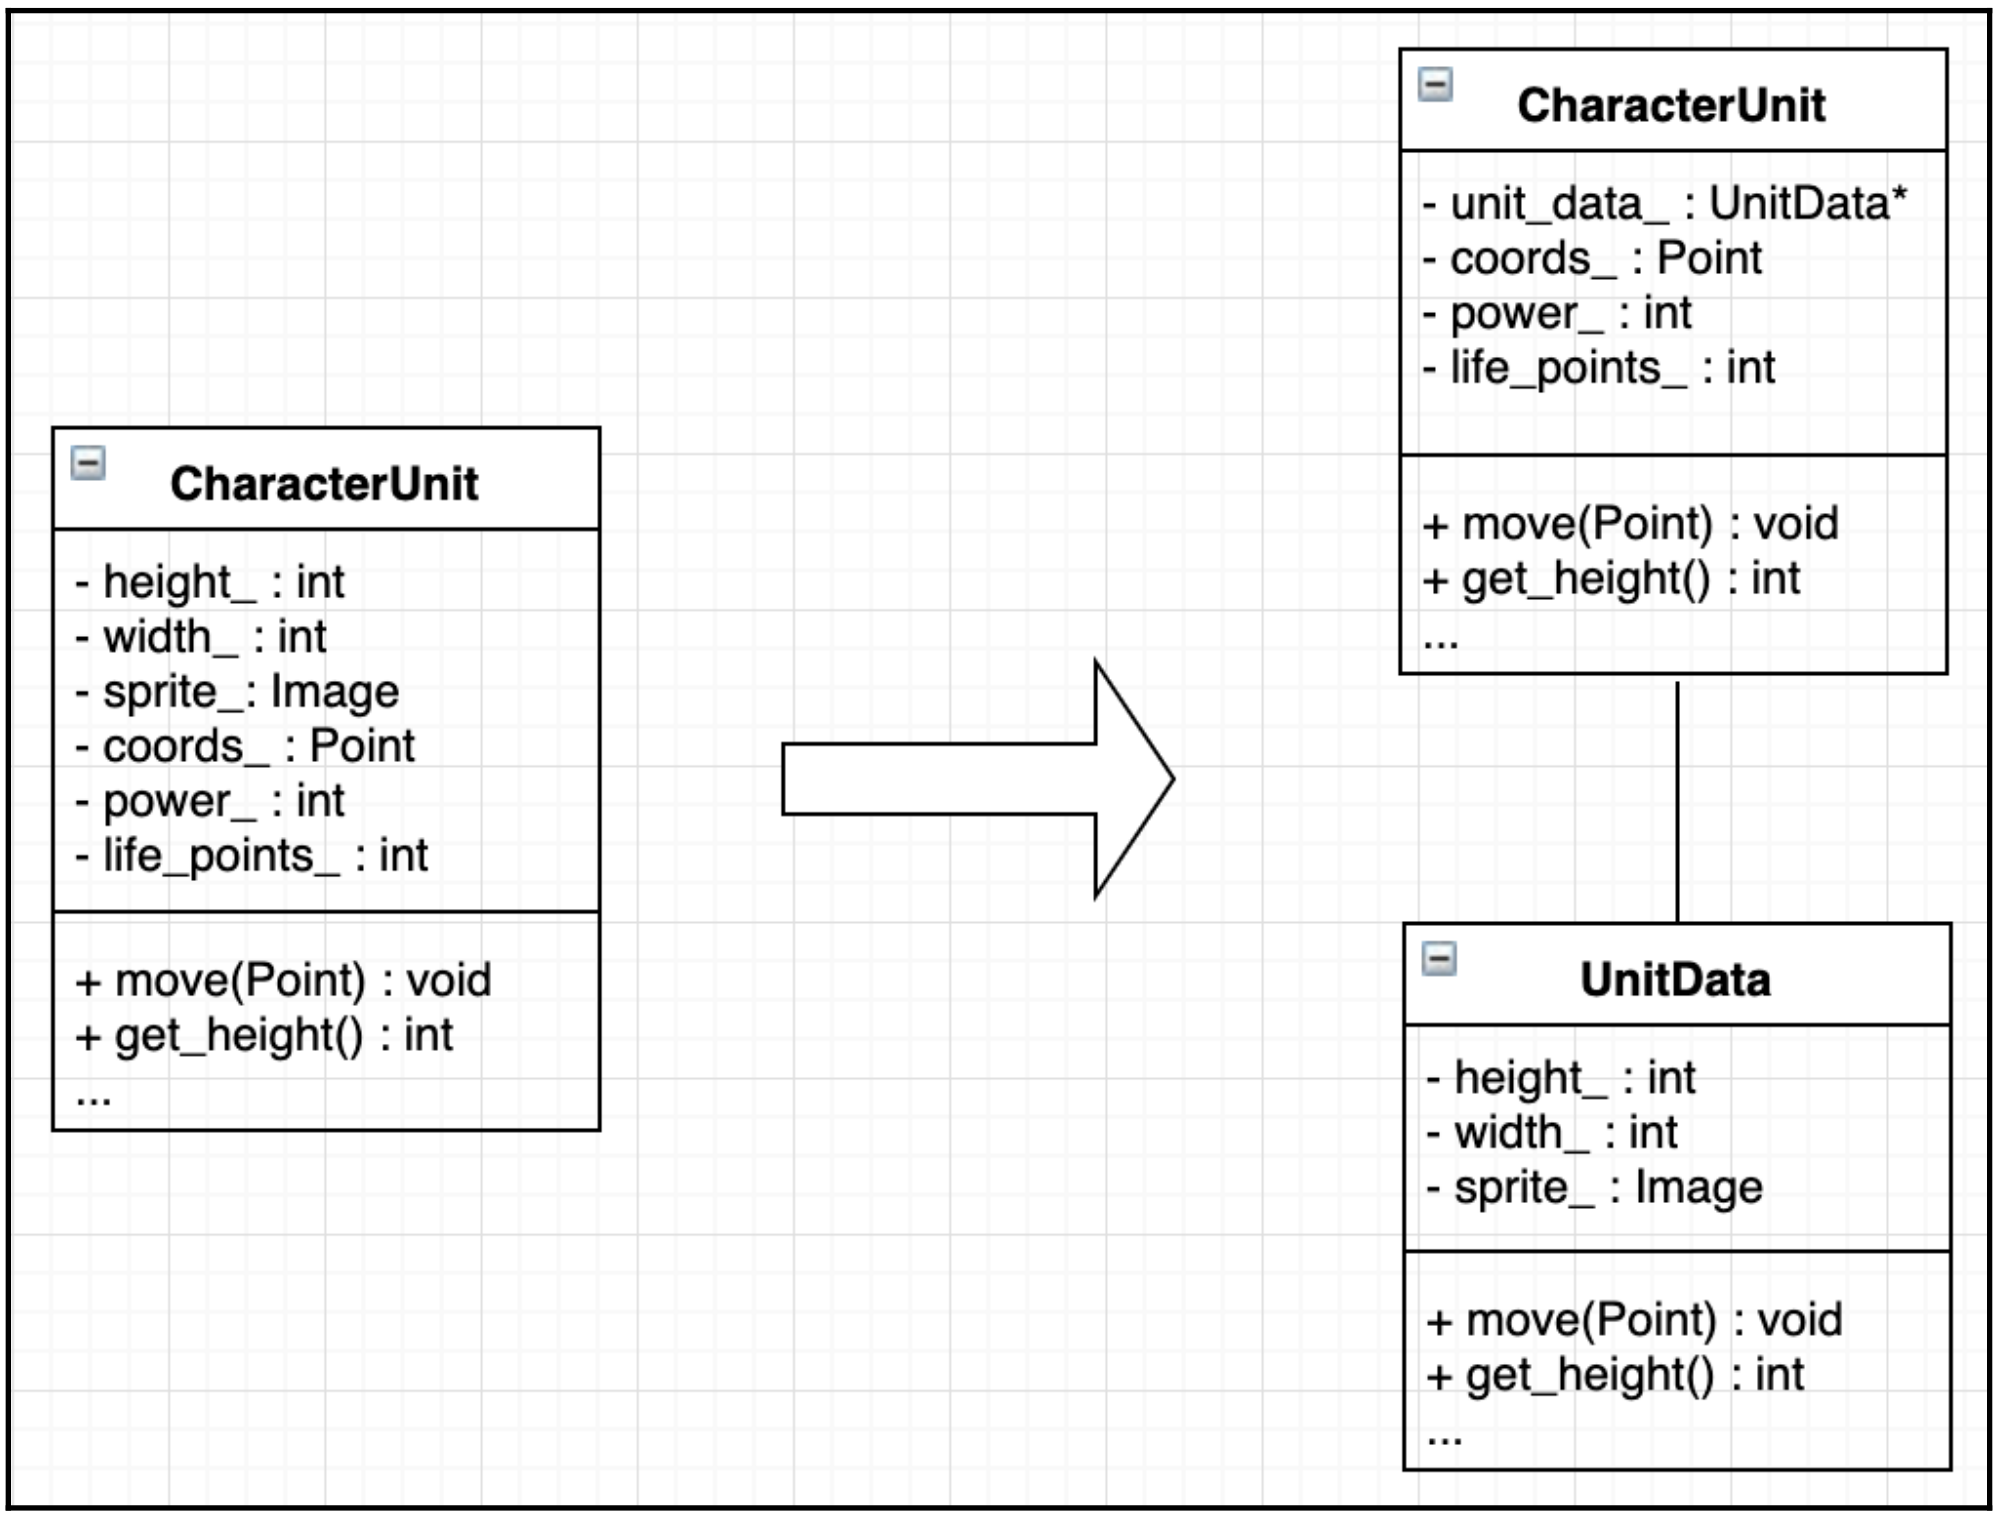
\includegraphics[width=1.0\textwidth]{content/Section-2/Chapter-11/11}
\end{center}

左边是修改前的CharacterUnit,而右边表示使用享元模式进行的最近的修改。游戏现在可以处理一堆CharacterUnit对象,而每一个都将存储一些UnitData对象的引用。这样,我们节省了很多内存。我们将每个单元唯一的值存储在CharacterUnit对象中。这些价值观会随着时间而改变。尺寸和精灵是恒定的,所以我们可以保持一个具有这些值的对象。这种不可变的数据称为内在状态,而对象的可变部分(CharacterUnit)称为外在状态。 \par
我们有意地将数据成员移动到CharacterUnit,从而将其从接口重新设计为抽象类。正如我们在第3章中所讨论的,抽象类几乎与可能包含实现的接口相同。move()方法是所有类型单元的默认实现的。因为所有的单元都有共同的属性,派生类只提供必要的行为就好,比如:生命点和能量。 \par
优化内存使用之后,我们应该处理复制对象。这款游戏涉及大量创造新对象。每个建筑都产生一个特定的角色单位,角色单位建造建筑,游戏世界本身呈现装饰元素(树木、岩石等)。现在,让我们尝试通过合并克隆功能来改进CharacterUnit。在本章的前面,我们故意删除了复制构造函数和赋值操作符。现在,是时候提供一种从现有对象创建新对象的机制了。 \par

\noindent\textbf{}\ \par
\textbf{原型模式} \ \par
该模式允许我们独立于对象类型创建对象的副本。下面的代码代表了关于我们最近修改的CharacterUnit类的最终版本。我们还将添加新的clone()成员函数,以合并原型模式: \par

\begin{lstlisting}[caption={}]
class CharacterUnit
{
public:
	CharacterUnit() {}
	CharacterUnit& operator=(const CharacterUnit&) = delete;
	virtual ~Character() {}
	virtual CharacterUnit* clone() = 0;
	
public:
	void move(const Point& to) {
		// the graphics-specific implementation
	}
	virtual void attack(const CharacterUnit&) = 0;
	virtual void destroy() = 0;
	int get_power() const { return power_; }
	int get_life_points() const { return life_points_; }
	
private:
	CharacterUnit(const CharacterUnit& other) {
		life_points_ = other.life_points_;
		power_ = other.power_;
	}

private:
	int life_points_;
	int power_;
};
\end{lstlisting}

我们删除了赋值操作符,并将复制构造函数移动到private部分。派生类覆盖clone()成员函数,如下所示: \par

\begin{lstlisting}[caption={}]
class Reader : public CharacterUnit
{
public:
	Reader* clone() override {
		return new Reader(*this);
	}

	// code omitted for brevity
};
\end{lstlisting}

原型模式将复制委托给对象。公共接口允许我们将客户端代码与对象的类解耦。现在,我们可以在不知道它是读者或士兵的情况下,复制一个角色单位。请看下面的例子: \par

\begin{lstlisting}[caption={}]
// The unit can have any of the CharacterUnit derived types
CharacterUnit* new_unit = unit->clone();
\end{lstlisting}

当需要将对象转换为特定类型时,要强制将工作动态转换为良好。 \par
在本节中,我们讨论了许多有用的设计模式。如果你不熟悉这些模式,这似乎有点难以应付,正确使用它们可以让我们设计灵活和可维护的项目。最后让我们回到我们之前介绍的游戏循环。 \par

\noindent\textbf{}\ \par
\textbf{设计游戏循环} \ \par
策略游戏的玩法变化最大。在每一个时间点上,许多动作同时发生。读者完成了他们的建筑,兵营生士兵,士兵攻击敌人,玩家命令单位移动、建造、攻击或奔跑等。游戏循环处理一切。通常,游戏引擎提供设计良好的游戏循环。 \par
游戏循环在我们玩游戏时运行。正如我们已经提到的,循环处理玩家的动作,更新游戏状态,并呈现游戏(让玩家可以看到状态变化)。它在每次迭代中都这样做。循环还应该控制游戏玩法的速率,也就是FPS。例如,如果你设计一款以60帧每秒运行的游戏,这意味着每帧大约需要16毫秒。 \par
以下代码是在本章前面的简单游戏循环中使用的: \par

\begin{lstlisting}[caption={}]
while (true)
{
	processUserActions();
	updateGame();
}
\end{lstlisting}

如果没有需要处理的用户操作,上述代码将快速运行。它在速度较快的机器上运行得更快(目标是坚持16毫秒每帧)。这可能需要我们在处理动作和更新游戏状态后等待一段时间,如下图所示: \par

\begin{center}
	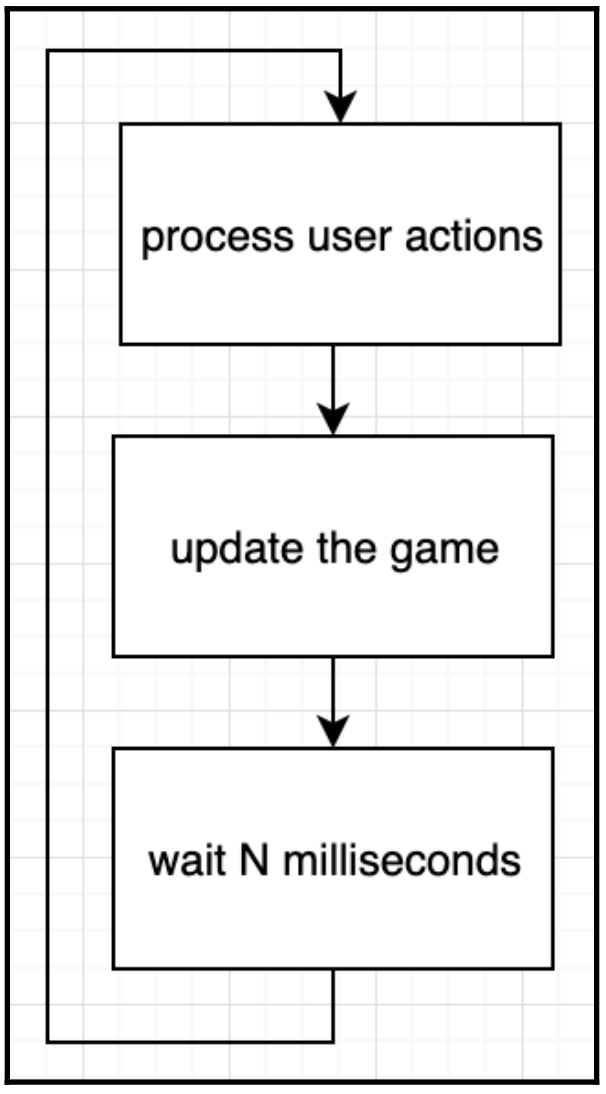
\includegraphics[width=0.4\textwidth]{content/Section-2/Chapter-11/12}
\end{center}

每次更新都将游戏时间提前一个固定的时间,这需要在现实世界中处理一个固定的时间。另一方面,如果一个帧的处理时间超过了指定的毫秒,游戏就会变慢。 \par
如上图所示,游戏中发生的所有事情都包含在游戏的更新部分中。大多数时候,更新可能需要一次执行多个操作。此外,我们必须为游戏后台发生的一些操作保留计时器,这主要取决于游戏的细节。例如,建造一座建筑可以表现为两种状态:初始状态和最终状态。 \par
在平面设计上,这两种状态应该代表两种不同的图像。第一张图片包含了建筑的一些基本部分,可能还包括一些围绕它的岩石,就好像它正在准备被建造一样。下一个图像代表了最终建成的建筑。当角色单位开始建造建筑时,我们便会向玩家呈现第一张图像(注:即围绕着一些岩石的基座)。当建筑完成后,我们用包含最终建筑的图像替换第一张图像。为了使这个过程更自然(更真实),我们人为地延长了时间。这意味着我们在图像的两个状态之间保持一个持续30秒或更多的计时器。 \par
我们用最少的细节描述了最简单的情况。如果我们需要让游戏变得更加详细,例如:通过渲染建筑在建造过程中的每个变化,我们就应该在代表建筑每个步骤的图像之间保留大量计时器。在更新游戏后,我们等待N毫秒。等待更多毫秒会让游戏流程更接近现实生活。如果更新时间太长,导致玩家体验滞后怎么办?在这种情况下,我们需要优化游戏,使其符合用户的最佳体验。现在,假设更新游戏需要执行数百次操作,玩家实现了一个繁荣的帝国,现在正在建造许多建筑物,并且用许多士兵攻击敌人。 \par
一个角色单位的每个行动,如从一个点移动到另一个点,攻击一个敌人单位,建造一座建筑等,都会在屏幕上及时呈现。现在,如果我们一次在屏幕上渲染数百个单位的状态会怎样?这就是我们使用多线程方法的地方。每个行动都涉及独立修改对象(注:对象是游戏中的任何单位,包括静态建筑)的状态。 \par

\noindent\textbf{}\ \par
\textbf{总结} \ \par
设计游戏是一项复杂的任务。我们可以将游戏开发视为一个独立的编程领域。游戏有不同的类型,其中之一就是策略游戏。策略游戏设计包括设计单位和建筑等游戏组件。通常情况下,策略游戏包括收集资源、建立帝国和与敌人战斗。游戏玩法包括游戏组件之间的动态交流,如角色单位建造建筑和收集资源,士兵防御敌人的土地等。 \par
为了恰当地设计一款策略游戏,我们结合了OOP设计技巧和设计模式。设计模式在设计整个游戏及其组件的交互过程中扮演着重要角色。在本章中,我们讨论了命令模式,它将动作封装在对象中;观察者模式,用于关注对象事件;以及中介模式,该模式用于将观察者推进到组件之间复杂交互的级别。  \par
游戏最重要的部分是它的循环。游戏循环控制渲染、游戏状态的及时更新和其他子系统。设计它涉及到使用事件队列和计时器。现代游戏使用网络,允许多个玩家通过互联网一起玩游戏。 \par
在下一章中,我们将介绍C++的网络编程,这样你就能将网络整合到你的游戏中。 \par

\noindent\textbf{}\ \par
\textbf{问题} \ \par
\begin{enumerate}
	\item 重写一个私有虚拟函数的目的是什么?
	\item 描述命令设计模式。
	\item 享元模式如何节省内存使用?
	\item 观察者模式和中介模式之间有什么区别?
	\item 为什么我们要将游戏循环设计成一个无限循环?
\end{enumerate}

\noindent\textbf{}\ \par
\textbf{扩展阅读} \ \par
\begin{itemize}
	\item Game Development Patterns and Best Practices: Better games, less hassle by John P.Doran, Matt Casanova:  https:/​/​www.​amazon.​com/​Game-​Development-​Patterns-	Best-​Practices/​dp/​1787127834/​ .
\end{itemize}

\newpage









